\documentclass[t, screen, aspectratio=43]{beamer}
\usepackage[T1]{fontenc}
\usepackage[utf8]{inputenc}
\usepackage{epsf}
\usepackage{graphicx}
\usepackage{geometry}
\usepackage{tabularx}
\usepackage[table]{colortbl}
\usepackage{xcolor}
\usepackage{soul}
\usepackage[normalem]{ulem}
\usepackage{tikz}
\usepackage{subcaption}
% Use the NTNU-temaet for beamer 
% \usetheme[style=ntnu|simple|vertical|horizontal, 
%     language=bm|nn|en, 
%     smalltitle, 
%     city=all|trondheim|alesund|gjovik]{ntnu2017}
\usetheme[style=helvet,language=en]{ntnu2017}

\usepackage[english]{babel}
\usepackage[style=numeric,backend=biber,natbib=false,sorting=none]{biblatex}

\title[Short title]{Ultra low power integer-N ADPLL}
\subtitle{Master's thesis project - meeting 2}
\author[C Nielsen]{Cole Nielsen}
\institute[NTNU]{Department of Electronic Systems, NTNU}
\date{24 January 2020 (calendar week 4)}
%\date{} % To have an empty date

\addbibresource{example.bib} % Add bibliography database

% Set the reference style to numeric.
% See here: http://tex.stackexchange.com/questions/68080/beamer-bibliography-icon
\setbeamertemplate{bibliography item}[text] 

% Set bibliography fonts to a small size.
\renewcommand*{\bibfont}{\footnotesize}




\begin{document}

\begin{frame}
	\titlepage%
\end{frame}

% Alternatively, special title page command to get a different background
% \ntnutitlepage

% #############################################################################
% This week
% #############################################################################



% #############################################################################
% Timeline
% #############################################################################

\begin{frame}
	\frametitle{Time plan (pt. 1)}
	\begin{table}[htb!]
		\tiny
		\centering
		\vspace{-1em}
		\def\arraystretch{1.5}		
		\setlength\arrayrulewidth{0.75pt}
		\setlength{\tabcolsep}{1em} % for the horizontal padding
		\begin{tabular}{|c|l|l|l|}
			\hline 
			\rule[-1ex]{0pt}{2.5ex}\cellcolor{gray!40}\textbf{Week \#} & \cellcolor{gray!40}\textbf{Dates} &\cellcolor{gray!40}\textbf{Tasks} & \cellcolor{gray!40}\textbf{Outcomes}\\ 
			\hline 
			% \rule[-1ex]{0pt}{2.5ex} \cellcolor{green!20}\textbf{3}&\cellcolor{green!20}13.1 - 19.1 &\cellcolor{green!20}Review PLL Design &\cellcolor{green!20}Refreshed Knowledge\\ 
			% \hline 
			\rule[-1ex]{0pt}{2.5ex}\cellcolor{green!40}\textbf{4}&\cellcolor{green!40}20.1 - 26.1 &\cellcolor{green!40}Finalize high level modeling &\cellcolor{green!40}Component level specification\\ 
			\hline 
			\rule[-1ex]{0pt}{2.5ex}\textbf{5}& 27.1 - 2.2 & Establish test bench in Virtuoso & With ideal PLL implementation\\ 
			\hline 
			\rule[-1ex]{0pt}{2.5ex}\textbf{6}& 3.2 - 9.2& Schem. design: phase detector & TDC - flash and counter based \\ 
			\hline 
			\rule[-1ex]{0pt}{2.5ex}\textbf{7}& 10.2 - 16.2& Schem. design: phase detector & Bang-bang phase detector\\ 
			\hline 
			\rule[-1ex]{0pt}{2.5ex}\textbf{8}&17.2 - 23.2& RTL, synthesis, place\&route & Digital loop filter\\ 
			\hline 
			\rule[-1ex]{0pt}{2.5ex}\textbf{9}&24.2 - 1.3& RTL, synthesis, place\&route & Digital loop filter\\ 
			\hline 
			\rule[-1ex]{0pt}{2.5ex}\textbf{10}&2.3 - 8.3& Schem. design: oscillator & Ring DCO\\ 
			\hline 
			\rule[-1ex]{0pt}{2.5ex}\textbf{11}&9.3 - 15.3& Schem. design: oscillator & LC DCO\\ 
			\hline 
			\rule[-1ex]{0pt}{2.5ex}\textbf{12}&16.3 - 22.3& Schem. design: divider  &TSPC + pulse swallow or sync counter?\\ 
			\hline 
			\rule[-1ex]{0pt}{2.5ex}\textbf{13}&23.3 - 29.3&Schem. design: Calibration& RTL/schem. for calibration\\ 
			\hline 
			\rule[-1ex]{0pt}{2.5ex}\textbf{14}& 30.3 - 5.4 &  Flex week - schem. design & Finalize schematic level design\\ 
			\hline 
			\rule[-1ex]{0pt}{2.5ex}\textbf{15}& 6.4 - 12.4& {\color{red}\textbf{Easter}} & - \\ 
			\hline 
			\rule[-1ex]{0pt}{2.5ex}\textbf{16}& 13.4 - 19.4& Layout & Phase detector\\ 
			\hline 
			\rule[-1ex]{0pt}{2.5ex}\textbf{17}& 20.4 - 26.4& Layout & Oscillator\\ 
			\hline 
		\end{tabular}
		\begin{flushleft}\textbf{Legend:} \colorbox{red!20}{\textbf{Done}} \colorbox{green!20}{\textbf{Current}}  \colorbox{blue!20}{\textbf{Revised}}
		% *I will write the report simultaneously with the work.
		\end{flushleft}
		% \caption{Assigned specifications for branch line hybrid design.}
		% \label{asgn_specs}
	\end{table}   
\end{frame}

\begin{frame}
	\frametitle{Time plan (pt. 2)}
	\begin{table}[htb!]
		\tiny
		\centering
		\vspace{-1em}
		\def\arraystretch{1.5}		
		\setlength\arrayrulewidth{0.75pt}
		\setlength{\tabcolsep}{1em} % for the horizontal padding
		\begin{tabular}{|c|l|l|l|}
			\hline 
			\rule[-1ex]{0pt}{2.5ex}\cellcolor{gray!40}\textbf{Week \#} & \cellcolor{gray!40}\textbf{Dates} &\cellcolor{gray!40}\textbf{Tasks} & \cellcolor{gray!40}\textbf{Outcomes}\\ 
			\hline 
			\rule[-1ex]{0pt}{2.5ex}\textbf{18}& 27.4 - 3.5 & Layout & Divider/calibration\\ 
			\hline 
			\rule[-1ex]{0pt}{2.5ex}\textbf{19}& 4.5 - 10.5 & Layout & Finalization/system integration\\ 
			\hline 
			\rule[-1ex]{0pt}{2.5ex}\textbf{20}& 11.5 - 17.5 & Flex week (layout) OR yield improvement & Depending on progress\\ 
			\hline 
			\rule[-1ex]{0pt}{2.5ex}\textbf{21}& 18.5 - 24.5& {\color{blue}\textbf{Report writing}} & \\ 
			\hline 
			\rule[-1ex]{0pt}{2.5ex}\textbf{22}& 25.5 - 31.5& {\color{blue}\textbf{Report writing}} & \\ 
			\hline 
			\rule[-1ex]{0pt}{2.5ex}\textbf{23}& 1.6 - 7.6& {\color{blue}\textbf{Report writing}} & {\color{red}\textbf{Deadline 8.6}}\\ 
			\hline 
		\end{tabular}
		\begin{flushleft}\textbf{Legend:} \colorbox{red!20}{\textbf{Done}} \colorbox{green!20}{\textbf{Current}}  \colorbox{blue!20}{\textbf{Revised}}
		% *I will write the report simultaneously with the work.
		\end{flushleft}
		% \caption{Assigned specifications for branch line hybrid design.}
		% \label{asgn_specs}
	\end{table}   
\end{frame}




% #############################################################################
% This week
% #############################################################################


% #############################################################################
% Physical limits
% #############################################################################

\begin{frame}
	\frametitle{Defining PLL Requirements}
	\begin{block}{Radio application BER requirements.}
	\begin{minipage}{5cm}
		\begin{itemize}
			\scriptsize
			\item Simulated BER of GFSK radio with BT=0.3, 1 MSymbols/s, $\pm$ 250 kHz frequency deviation, 4 bit averaging in receiver for effective 250 kbps rate.
			\item Carrier to noise ratio (CNR) of the signal entering the demodulator greatly decreases after 6 dB (BER = $10^{-2}$ is at 5.1 dB). THUS targeting > 6 dB CNR.
			\item CNR $\approx$ Residual phase modulation (i.e. integrated phase noise power).
		\end{itemize} 	
	\end{minipage}
	\begin{minipage}{6cm}
		\vspace{1em}
		\hspace{1em}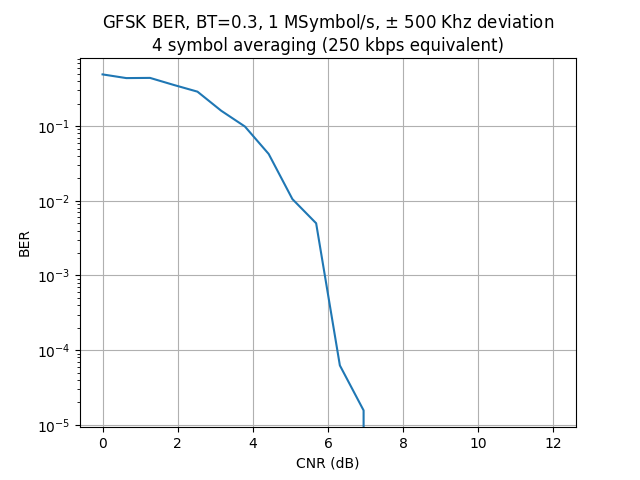
\includegraphics[width=1\textwidth, angle=0]{ber_curve.png}
	\end{minipage}
	\end{block}
\end{frame}

\begin{frame}
	\frametitle{Ring oscillator phase noise}
	\begin{block}{Theoretical limit applied}
		\scriptsize
		Ring oscillator phase noise limit from "Minimum Achievable Phase Noise of RC Oscillators", Navid et al. 2005:
		\begin{equation}
			PN_{min}(\Delta f)= 10\log 10\left(\frac{7.33k_BT}{P}\left(\frac{f_0}{\Delta f}\right)^2\right)
		\end{equation}
		\vspace{-.8em}\\
		If $f_0$ = 2.4 GHz, P = 50 $\mu$W, $\Delta f$= 1 MHz, T = 293 K, $\rightarrow$ \textbf{PN$_{min}$ = -84.7 dBc/Hz} \\
		-- This limit applied to the below FOM comparison (FOM PN=165 dB):
		\vspace{-1.5em}
		\center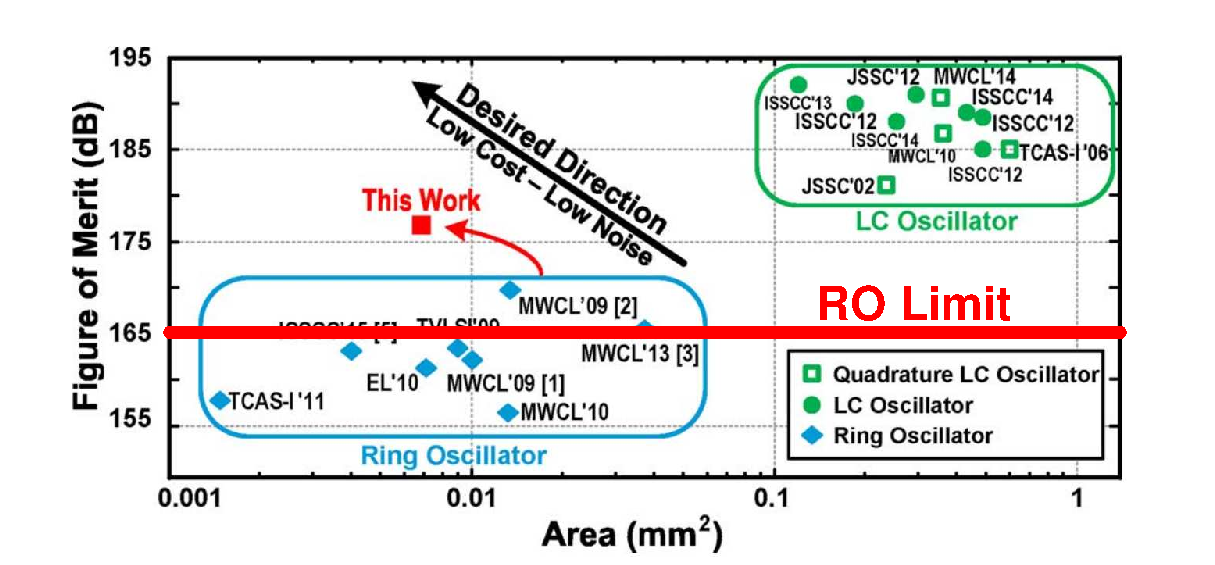
\includegraphics[width=0.75\textwidth, angle=0]{ro_perf.pdf}
	\end{block}
\end{frame}

\begin{frame}
	\frametitle{Simulated BER}
	\begin{block}{BBPD-optimized (total phase noise minimized).}
	\begin{minipage}{5cm}
		\begin{itemize}
			\scriptsize
			\item $f_0$ = 2.4 GHz, P = 50 $\mu$W, clock freq = 16 MHz.
			\item Optimized for minimum phase noise with BBPD. Closed loop BW = 911 kHz.
			\item \textbf{CNR = 26 dB}, low BER expected.
			\item Simulation recorded 0 BER (with 64000 bits)
		\end{itemize} 	
	\end{minipage}
	\begin{minipage}{6cm}
		\vspace{1em}
		\hspace{1em}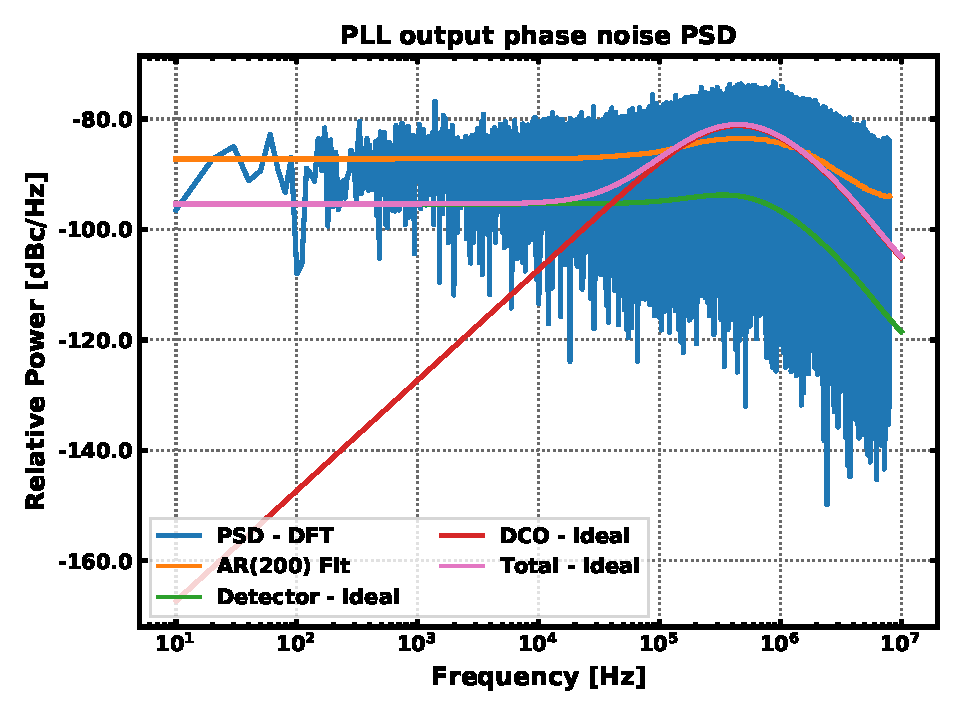
\includegraphics[width=1\textwidth, angle=0]{trans_phase_noise_fast.pdf}
	\end{minipage}
	\end{block}
\end{frame}

\begin{frame}
	\frametitle{Simulated BER}
	\begin{block}{Sub-optimal phase noise.}
	\begin{minipage}{5cm}
		\begin{itemize}
			\scriptsize
			\item $f_0$ = 2.4 GHz, P = 50 $\mu$W, clock freq = 16 MHz.
			\item Closed loop BW = 145 kHz.
			\item \textbf{CNR = 17 dB}
			\item Simulation recorded 0 BER (with 64000 bits)
			\item Even under non-optimal conditions, 50 $\mu$W provides >10 dB margin if 6 dB CNR is assumed limit.
		\end{itemize} 	
	\end{minipage}
	\begin{minipage}{6cm}
		\vspace{1em}
		\hspace{1em}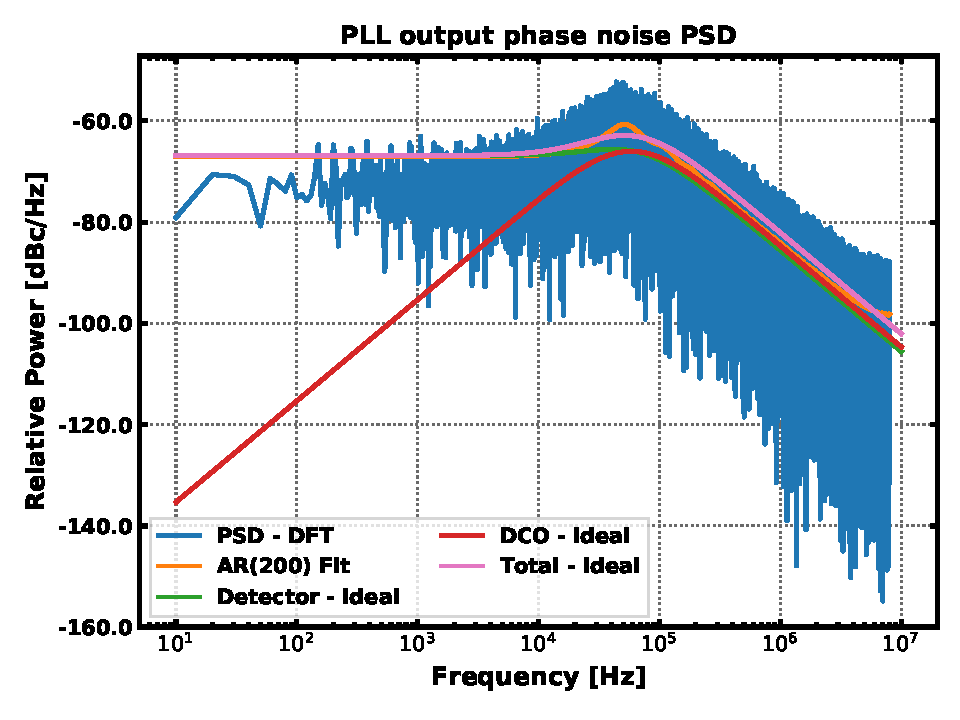
\includegraphics[width=1\textwidth, angle=0]{trans_phase_noise.pdf}
	\end{minipage}
	\end{block}
\end{frame}


% #############################################################################
% Loop Dynamics (continuous)
% #############################################################################

% \begin{frame}
% 	\frametitle{Loop Dynamics}
% 	\begin{block}{Still To Do}
% 		\vspace{-.2em}
% 		\begin{itemize}
% 			\footnotesize
% 			\item Standard approach to used mixed continuous/discrete time mathematical model for DPLL. 
% 			\item Plot of RO phase noise (typical)
% 			\item Automatic analysis of performance (lock detection, residual phase modulation, lock-in/pull-in range).
% 			\item Automatic optimization (using gradient descent) of PLL parameters?
% 			\item Z-domain modeling of loop? Develop (by hand) some ideal transfer funtions for loop.

% 		\end{itemize}    
% 	\end{block}
% \end{frame}

% #############################################################################
% Architecture - block diagram
% #############################################################################


\begin{frame}
	\frametitle{Architecture}
	\begin{block}{Block Diagram}
	\center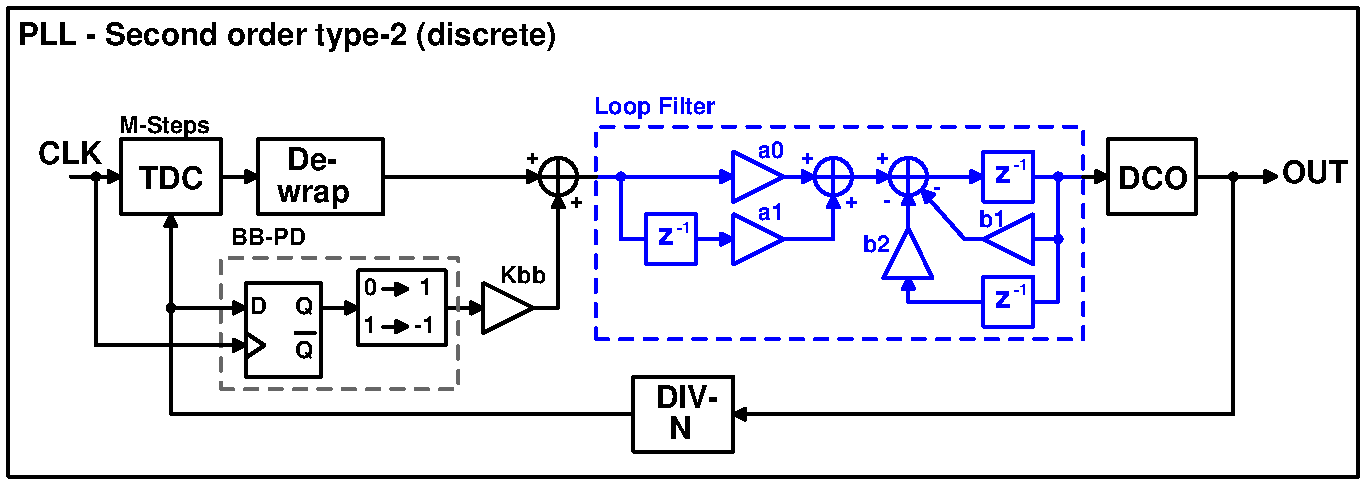
\includegraphics[width=0.8\textwidth, angle=0]{pll_sec_order_bb.pdf}

	\end{block}
		\begin{block}{Power Targets}
		\vspace{-.1em}
		\begin{table}[htb!]
			\tiny
			\centering
			\def\arraystretch{1.5}		
			\setlength\arrayrulewidth{0.75pt}
			\setlength{\tabcolsep}{1em} % for the horizontal padding
			\begin{tabular}{|l|l|l|l|l|l|}
				\hline 
				\rule[-1ex]{0pt}{2.5ex} \cellcolor{gray!40}\textbf{DCO} & \cellcolor{gray!40}\textbf{Phase detector} & \cellcolor{gray!40}\textbf{Divider }& \cellcolor{gray!40}\textbf{Digital (LF)}& \cellcolor{gray!40}\textbf{Other} & \cellcolor{gray!40}\textbf{SUM} \\ 
				\hline 
				\rule[-1ex]{0pt}{2.5ex} 50 $\mu$W& 10 $\mu$W & 10 $\mu$W & 10 $\mu$W  & $<<$ 10 $\mu$W & $<$ 100 $\mu$W\\ 
				\hline 
			\end{tabular} 
			% \caption{Assigned specifications for branch line hybrid design.}
			% \label{asgn_specs}
		\end{table}   
	\end{block}

\end{frame}

% #############################################################################
% Specification
% #############################################################################

\begin{frame}
	\frametitle{Specification\color{black}}
	\begin{block}{System Performance Targets}
		\scriptsize
		\begin{table}[h!]
			\centering
			\def\arraystretch{1.5}		
			\setlength\arrayrulewidth{0.75pt}
			\setlength{\tabcolsep}{1em} % for the horizontal padding
			\begin{tabular}{|l|r|l|l|}
				\hline 
				\rule[-1ex]{0pt}{2.5ex} \cellcolor{gray!40}\textbf{Parameter} & \cellcolor{gray!40}\textbf{Value} & \cellcolor{gray!40}\textbf{Unit }& \cellcolor{gray!40}\textbf{Notes}\\ 
				\hline 
				\rule[-1ex]{0pt}{2.5ex} \textbf{Frequency}  & 2.4-2.4835 & GHz & 2.4G ISM Band\\ 
				\hline 
				\rule[-1ex]{0pt}{2.5ex} \textbf{Ref. frequency} & 16 & MHz & Yields 6 channels \\ 
				\hline 
				\rule[-1ex]{0pt}{2.5ex} \textbf{Power} & $\leq$ 100  &$\mu$W & minimize!\\ 
				\hline 
				\rule[-1ex]{0pt}{2.5ex} \textbf{FSK BER} & $\leq$ 1e-2  & & 2FSK with $f_{dev}$=$\pm$250 KHz\\ 
				\hline 
				\rule[-1ex]{0pt}{2.5ex} \cellcolor{yellow}\textbf{CNR} &\cellcolor{yellow} $<<$\cellcolor{yellow} 6 &\cellcolor{yellow} dB&\cellcolor{yellow} \\ 
				\hline 
				\rule[-1ex]{0pt}{2.5ex} \textbf{Initial Lock Time} & $\leq$ 10 & $\mu$s & Upon cold start \\ 
				\hline 
				\rule[-1ex]{0pt}{2.5ex} \textbf{Re-lock Time} & $\leq$ 5 & $\mu$s & Coming out of standby \\ 
				\hline 
				\rule[-1ex]{0pt}{2.5ex} \textbf{Lock $\Delta f$ tolerance} & $10^5$ & Hz& \\ 
				\hline 
			\end{tabular} 
			% \caption{Assigned specifications for branch line hybrid design.}
			% \label{asgn_specs}
		\end{table}   
		Additionally: PLL output should support IQ sampling at LO frequency.
	\end{block}    
\end{frame}

\begin{frame}
	\frametitle{Specification\color{black}}
	\begin{block}{Component-level specs}
		\scriptsize
	\begin{table}[h!]
		\centering
		\def\arraystretch{1.5}		
		\setlength\arrayrulewidth{0.75pt}
		\setlength{\tabcolsep}{1em} % for the horizontal padding
		\begin{tabular}{|l|r|l|}
			\hline 
			\rule[-1ex]{0pt}{2.5ex} \cellcolor{gray!40}\textbf{Parameter} & \cellcolor{gray!40}\textbf{Value} & \cellcolor{gray!40}\textbf{Unit }\\ 
			\hline 
			\rule[-1ex]{0pt}{2.5ex} \textbf{Counter range}  & 256 steps & coverage of 150-155 \\ 
			\hline 
			\rule[-1ex]{0pt}{2.5ex} \textbf{Divider ratio} & 150-155  & (For non-counter based)\\ 
			\hline 
			\rule[-1ex]{0pt}{2.5ex} \textbf{TDC resolution} &$\geq$ 155  & steps/reference cycle\\ 
			\hline 
			\rule[-1ex]{0pt}{2.5ex} \textbf{DCO gain $K_{DCO}$} & $10^4$ & Hz/LSB \\ 
			\hline 
			\rule[-1ex]{0pt}{2.5ex} \textbf{DCO Phase noise} &$<$ -80 & dBc/Hz at $\Delta f=10^6$ Hz \\ 
			\hline 
			\rule[-1ex]{0pt}{2.5ex} \textbf{DCO Power} & $\leq$ 50 & $\mu$W \\ 
			\hline 
			\rule[-1ex]{0pt}{2.5ex} \textbf{Digital filter word resolution} & 13 & bits \\ 
			\hline 
		\end{tabular} 
		% \caption{Assigned specifications for branch line hybrid design.}
		% \label{asgn_specs}
		\caption{System-level specifications}
		\label{design_specs}
	\end{table}   
	\end{block}    
\end{frame}

% #############################################################################
% project phases
% #############################################################################

% ############################################################################b#
% References
% #############################################################################


% \begin{frame}
% 	\frametitle{References}
% 		\scriptsize
% 		[1] "Ultra-Low Power Wake-Up Receivers for Wireless Sensor Networks", N. Pletcher, J.M Rabaey, 2008.\\
% 		\hspace{16pt}\url{http://www.eecs.berkeley.edu/Pubs/TechRpts/2008/EECS-2008-59.html}\\
% 		\vspace{1em}
% 		% [2] "Minimum Achievable Phase Noise of RC Oscillators",
% 	% Navid et al. 2005
% \end{frame}


\end{document}
